%!TEX program = xelatex
\documentclass{article}

\usepackage[T1]{fontenc}
\usepackage[polish]{babel}
\usepackage[utf8]{inputenc}
\usepackage{titling}
\usepackage{multicol}
\usepackage{paracol}
\usepackage{indentfirst}
\usepackage{float}

\usepackage[utf8]{inputenc} %rodzaj czcionki w dokumencie
\usepackage{geometry} %poprawienie marginesów
\usepackage{polski} %polskie znaki
\usepackage{multirow} %tabela
\usepackage{graphicx} %tabela
\usepackage{float} %poprawienie pozycji
\usepackage{fancyhdr} % header i footer
\usepackage{karnaugh-map} % rysowanie siatek karnaugh
\usepackage{hyperref} %tworzenie odnośników, \url{<url>}, \href{<file path, link>}{<text with link>} \pageref{}
\usepackage{amsmath} % Matma
\usepackage{boldline}%edytowanie grubości krawędzi w tabelach \hlineB{} \clineB{}{}
\usepackage{array}%grubsze kolumny w tabeli
\usepackage{bigstrut}
\usepackage{caption}
\usepackage{listings} %pisanie kodu w ładny sposób, begin{listings}[language=<język>]...end{listings} tak samo jak nazwa paczki

\usepackage[letterpaper,top=2cm,bottom=2cm,left=3cm,right=3cm,marginparwidth=1.75cm]{geometry}

\usepackage{amsmath}
\usepackage{graphicx}
\usepackage[colorlinks=true, allcolors=blue]{hyperref}

%Ustawienie paczki hyperref
\hypersetup{
     colorlinks,
     citecolor=black,
     filecolor=black,
     linkcolor=black,
     urlcolor=black
	%  language=vhdl
}

\definecolor{backcolour}{rgb}{0.95,0.95,0.92}
\definecolor{AO}{rgb}{0,0.5,0}
\definecolor{ZeroBlue}{rgb}{0,0.28,0.73}
\definecolor{DarkRed}{rgb}{0.85,0.16,0.16}

\lstset{
breaklines=true,
language=vhdl,
numbers=left,
tabsize=2,
numberstyle=\tiny,
backgroundcolor=\color{backcolour},
breakatwhitespace=false,
showspaces=false,                
showstringspaces=false,
showtabs=false,
commentstyle=\color{gray},
keywordstyle=\color{ZeroBlue},
% keywordstyle={[2]\color{DarkRed}},
% keywordstyle={[3]\color{ZeroBlue}},
}


\begin{document}

\begin{titlepage}
    \begin{center}\LARGE POLITECHNIKA WROCŁAWSKA \\ WYDZIAŁ INFORMATYKI I TELEKOMUNIKACJI \end{center}
    \vspace{57pt}
    \begin{center} \Huge Układy cyfrowe i systemy wbudowane 2 \end{center}
    \vspace{35pt}
    \begin{center} \LARGE Instrument muzyczny \\ Sprawozdanie końcowe z projektu \end{center}
    \vspace{40pt}
    \begin{flushleft}\Large Termin zajęć: PON, 8:00-11:00 TP   \end{flushleft}
    \vspace{15pt}
    \begin{paracol}{2}
        \raggedright{\Large Autorzy (Grupa B):} \switchcolumn \raggedleft{\Large Prowadzący zajęcia:} \switchcolumn
        \raggedright{\Large Maciej Byczko, 252747} \switchcolumn \raggedleft{\Large dr inż. Jacek Mazurkiewicz} \switchcolumn
        \raggedright{\Large Bartosz Matysiak, 252757} 
    \end{paracol}
    \vspace{150pt}
    \begin{center}Wrocław, \the\year{}r.\end{center}
\end{titlepage}

%\tableofcontents

%\newpage

\section{Temat projektu}

Projekt miał dotyczyć wykonania implementacji w~sprzęcie instrumentu muzycznego typu ''keyboard'' przy użyciu płyty Spartan 3E.

\section{Opis funkcjonalności} % tą sekcję chyba zamienić w zwykły akapit

\subsection{Założenia początkowe}
W trakcie sporządzania początkowych założeń projektowych, stworzyliśmy następujące listy funkcjonalności:

\subsubsection{Wersja podstawowa}

\begin{itemize}
    \item Możliwość użycia gamy dźwięków uprzednio nagranych na kartę SD. 
    \item Wsparcie dla klawiatury komputerowej.
    \item Odtworzenie dźwięku.
\end{itemize} 

\subsubsection{Możliwe rozszerzenia}

\begin{itemize}
    \item Możliwość prostej syntezy jednotonowej.
    \item Wsparcie dla \href{https://pl.wikipedia.org/wiki/Launchpad}{launchpada}.
\end{itemize}

\subsection{Porównanie i nasza ocena projektu}
Udało się zrealizować wszystkie założenia wymienione na liście funkcjonalności podstawowych; efekty tej części naszej pracy uważamy za zadowalające, zgodne z naszymi pierwotnymi wyobrażeniami co do funkcjonowania projektu. Ze względu na niespodziewane problemy nie zdążyliśmy przystąpić do prac nad rozszerzeniami. Z całą pewnością, dysponując większą ilością czasu, wykonalibyśmy wymienione rozszerzenia w pierwszej kolejności.

\section{Schemat urządzenia}

\begin{figure}[H]
    \centering
    \resizebox*{\textwidth}{!}{
        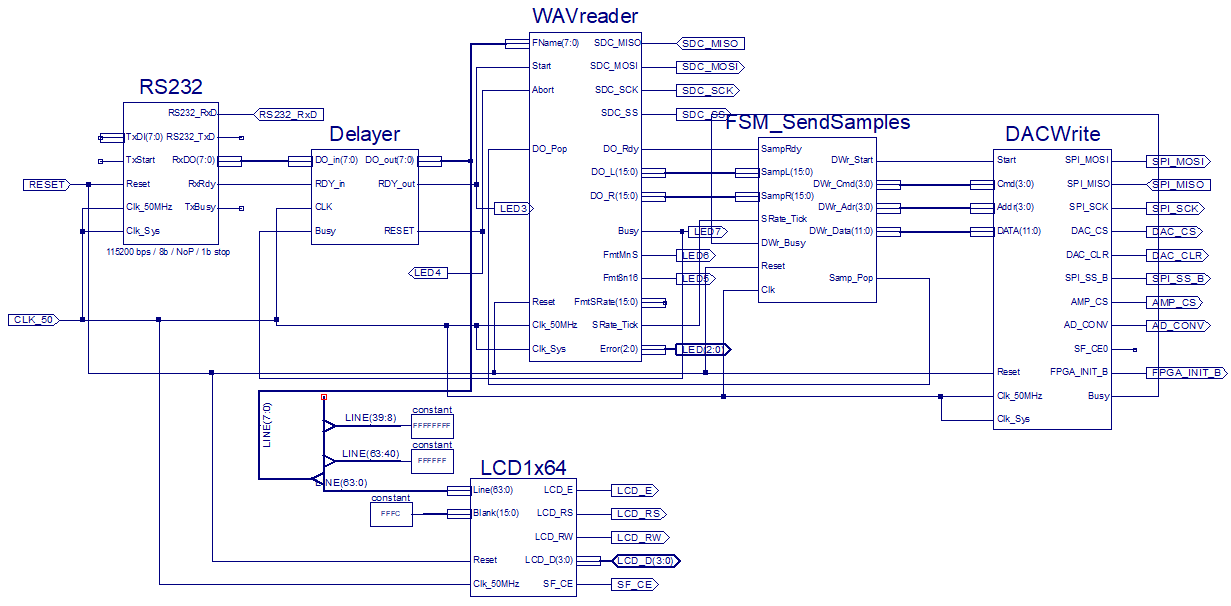
\includegraphics{schematic.png}
    }
\end{figure}

W projekcie wykorzystane zostały moduły własne, jak też te dostępne na stronie \href{http://www.zsk.ict.pwr.wroc.pl/zsk_ftp/fpga/#_Toc99974115}{Zestawu Digilent S3E-Starter}.
Poza modułami ukazanymi na schemacie, projekt wykorzystuje także dodatkowe urządzenia: kartę SD z systemem plików FAT32, klawiaturę na złącze RS232 oraz głośnik. Dodatkowo, informacje pomocnicze dotyczące prawidłowego działania układu ukazywane są na diodach LED oraz wyświetlaczu LCD.

\section{Podział projektu na moduły}

Listy modułów użytych w projekcie są kolejnym elementem, który uległ zmianie względem pierwotnych założeń:

\subsection{Wykorzystane moduły ze strony kursu}

\begin{itemize}
    \item \textbf{WAVreader} - obsługa karty SD 
    \item \textbf{RS232} - obsługa klawiatury PS2 
    \item \textbf{DACWrite} - obsługa głośnika
    \item \textbf{FSM\_SendSamples} - pomocnicza maszyna stanów
\end{itemize}

\subsection{Moduły własne, przygotowane na potrzeby projektu}

\begin{itemize}
    \item \textbf{Delayer} - moduł opóźniająco - przerywający do obsługi żądań odtwarzania dźwięków.
\end{itemize}

\subsection{Kody źródłowe i opisy modułów}

\subsubsection{Delayer}

\begin{figure}[H]
    \centering
    \resizebox*{\textwidth}{!}{
        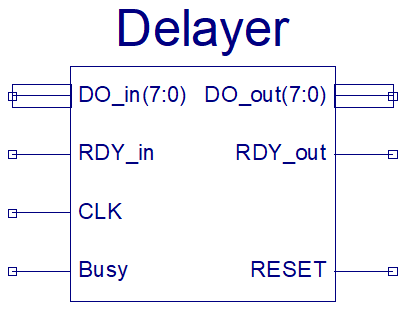
\includegraphics{delayer.png}
    }
\end{figure}

\lstinputlisting{Delayer.vhd}

Moduł służy do opóźniania sygnału \textbf{RxDO(7:0)} i został zrealizowany jako poniższa maszyna stanów:

\begin{figure}[H]
    \centering
    \resizebox*{\textwidth}{!}{
        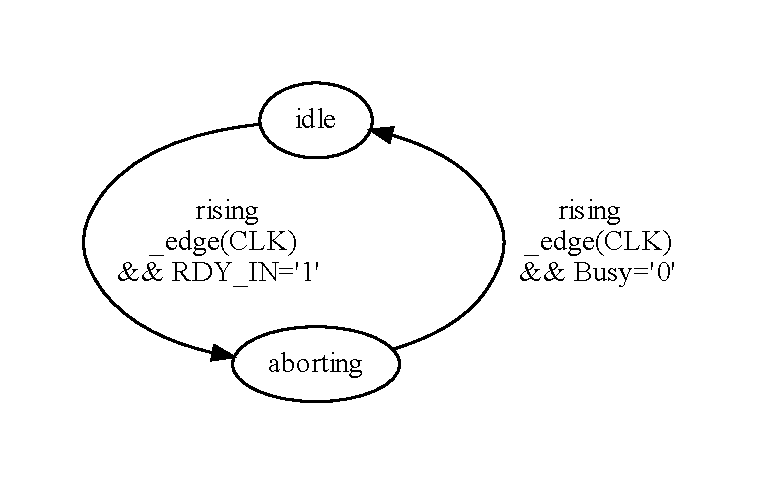
\includegraphics{delayer_state_machine.pdf}
    }
\end{figure}

Logiczna jedynka na wejściu \textbf{RDY\_IN} jest sygnałem powodującym przejście układu ze stanu \textit{idle} do stanu \textit{aborting} oraz ustawienie wyjścia \textbf{RESET}.
Powrót do stanu \textit{idle} następuje dopiero, gdy nastąpi zmiana na logiczne zero sygnału \textbf{Busy}, podanego jako sprzężenie zwrotne z układu \textbf{WAVreader}. Ma miejsce wtedy też wyzerowanie sygnału \textbf{RESET} i dopiero wtedy następuje podanie nowych wartości sygnałów \textbf{DO\_out(7:0)} i \textbf{RDY\_out}.

Sensem użycia modułu \textbf{Delayer} jest wspomożenie działania modułu \textbf{WAVreader}, który umożliwia przerwanie odtwarzania pliku, jednak powrót do stanu gotowości może i zazwyczaj nie jest natychmiastowy. 

\subsubsection{FSM\_SendSamples}

\begin{figure}[H]
    \centering
    \resizebox*{\textwidth}{!}{
        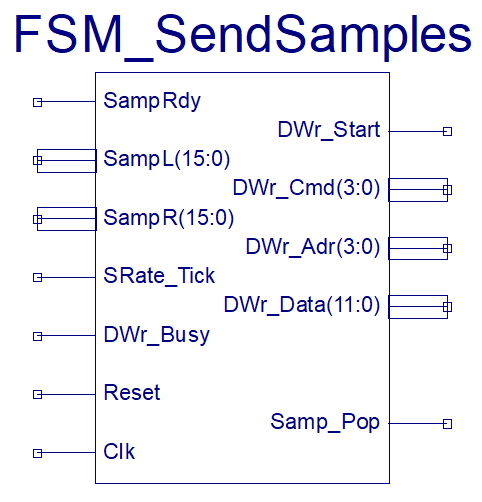
\includegraphics{fsm_send_samples.png}
    }
\end{figure}

\lstinputlisting{FSM_SendSamples.vhd}

Moduł pomocniczy ze strony kursu, sześciostanowa maszyna stanów służąca jako moduł wspomagający wysyłanie próbek do modułu \textbf{DACWrite}.

\subsection{Omówienie modułów - czarnych skrzynek} % jak wykorzystano 

\subsubsection{RS232}

\begin{figure}[H]
    \centering
    \resizebox*{0.8\textwidth}{!}{
        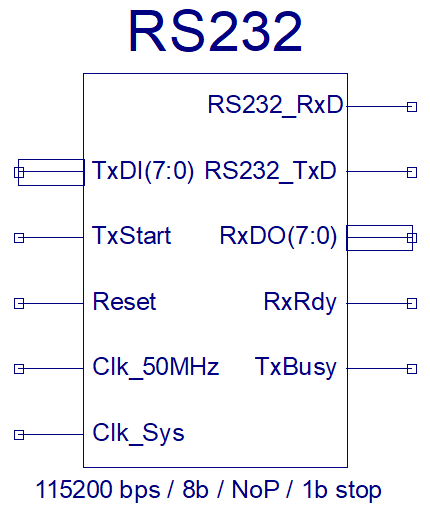
\includegraphics{RS232.png}
    }
\end{figure}

Moduł umożliwiający obsługę urządzeń podłączonych przez interfejs RS232. W projekcie wykorzystujemy go do odbioru bajtów, których źródłem jest klawiatura. Wyprowadzenia odpowiedzialne za wysył danych pozostają niewykorzystane.

\subsubsection{WAVreader}

\begin{figure}[H]
    \centering
    \resizebox*{0.5\textwidth}{!}{
        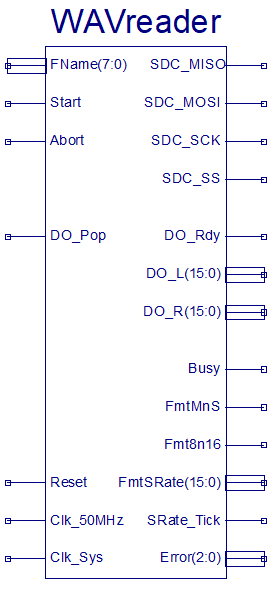
\includegraphics{WAVreader.png}
    }
\end{figure}

Moduł służący do obsługi karty SD; w momencie ustawienia jedynki na wejściu \textbf{Start} odczytywany jest kod ascii znaku z wejścia \textbf{FName}. Następnie plik o rozszerzeniu \textit{*.wav} i nazwie zadanej poprzez odczytany znak jest sczytywany z karty SD, a jego rozszerzone do 16 bitów próbki wysyłane na wyjścia \textbf{DO\_L} i \textbf{DO\_R}.
W projekcie wykorzystujemy także funkcjonalność jaką daje wejście \textbf{Abort} - umożliwia ono przerwanie odtwarzania danego pliku. O zakończeniu procesu przerywania i powrocie modułu do stanu podstawowego informuje nas zero logiczne na wyjściu \textbf{Busy}.

\subsubsection{DACWrite}

\begin{figure}[H]
    \centering
    \resizebox*{0.5\textwidth}{!}{
        \includegraphics{DACWrite.png}
    }
\end{figure}

Moduł obsługujący wysyłanie danych do przetwornika DAC LTC2624. W naszym projekcie wykorzystujemy go do obsługi głośnika.

\subsubsection{LCD1x64}

\begin{figure}[H]
    \centering
    \resizebox*{\textwidth}{!}{
        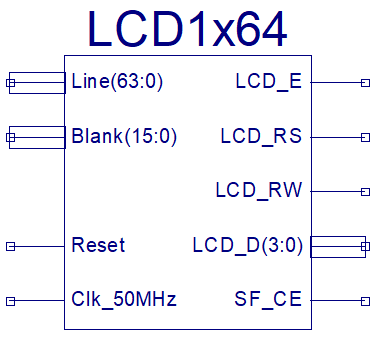
\includegraphics{LCD.png}
    }
\end{figure}

Moduł wspomagający testowanie urządzenia i jego testowanie; nie pełni żadnej innej istotnej roli w projekcie.

\section{Instrukcja obsługi urządzenia}

Do uruchomienia naszego urządzenia będą potrzebne:

\begin{itemize}
    \item Płytka rozwojowa Spartan 3E Starter Board wyposażona w slot do odczytu karty SD;
    \item Plik \textit{*.bit} z konfiguracją naszego urządzenia;
    \item Program \textit{jrs\_term.exe};
\end{itemize}

a także urządzenia zewnętrzne:

\begin{itemize}
    \item Klawiatura obsługująca interfejs RS232;
    \item Głośnik;
    \item Karta SD z plikami \textbf{*.wav};
\end{itemize}

Lista kroków:

\begin{enumerate}
    \item Wszystkie wymienione urządzenia należy podłączyć pod odpowiednie dla nich porty.
    \begin{itemize}
        \item W przypadku głośnika jest to podłączenie pod piny C oraz GND z lewej strony płytki.
        \item Kartę SD należy włożyć do odpowiedniego slotu; Należy wcześniej zadbać, aby była ona sformatowana w systemie FAT32; Odtwarzane z niej pliki \textit{*.wav} powinny mieć nazwę składającą się z jednej litery - jest to jednocześnie nazwa klawisza, który posłuży do jego odtworzenia.
        \item Klawiaturę należy podłączyć pod interfejs RS232.
    \end{itemize}
    \item Gdy wszystkie urządzenia są podłączone, należy wgrać plik konfiguracyjny \textit{instrument.bit} na płytkę.
    \item Naciśnięcie klawiszy na klawiaturze powinno spowodować odtworzenie odpowiedniego dźwięku.
\end{enumerate}

W testowanej przez nas konfiguracji przejęliśmy wykorzystanie następujących zakresów znaków:

\begin{itemize}
    \item \lbrack12345678\rbrack - skrzypce;
    \item \lbrack qwertyui\rbrack - pianino;
    \item \lbrack asdfghjk\rbrack - syntezator;
\end{itemize}

Użytkownik może jednak całkowicie to zignorować i nagrać własne próbki dźwiękowe.

\begin{figure}[H]
    \centering
    \resizebox*{\textwidth}{!}{
        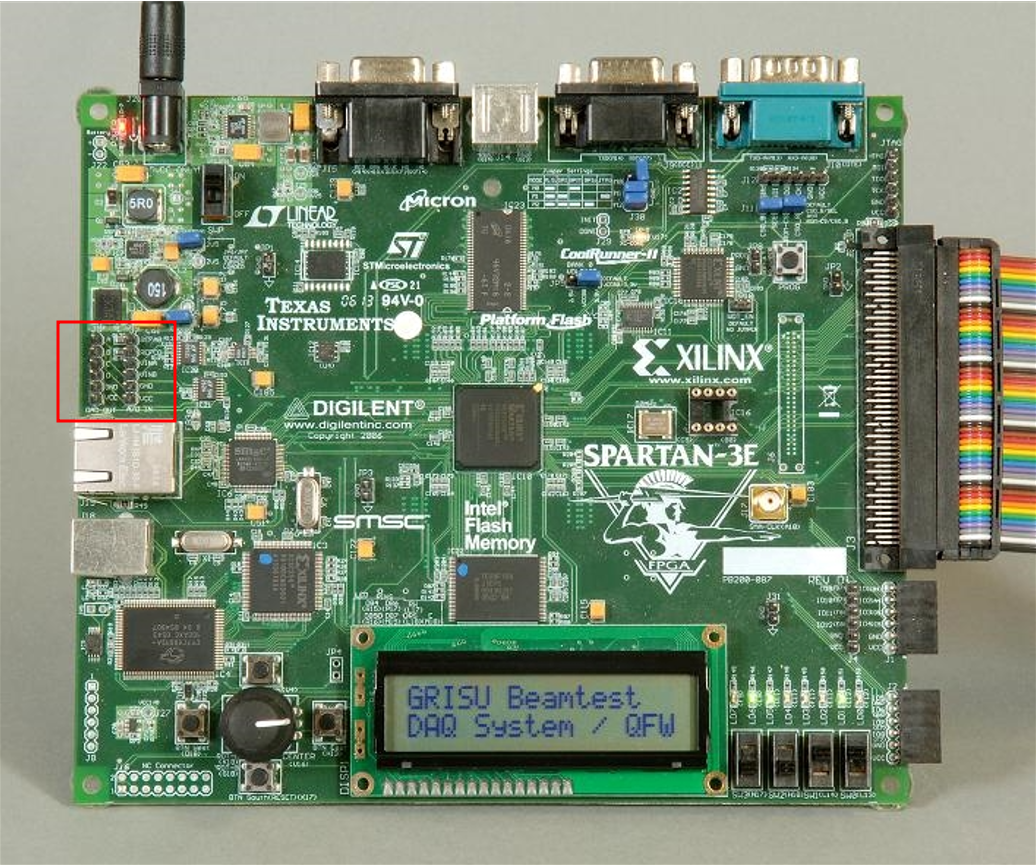
\includegraphics{podlaczenie_glosnika.png}
    }
    \caption{Miejsce podłączenia głośnika}
\end{figure}

\section{Literatura}

\begin{itemize}
    \item The Programmable Logic Data Book. Xilinx, Inc.
    \item Libraries Guide. Xilinx, Inc.
    \item http://www.zsk.ict.pwr.wroc.pl/zsk\_ftp/fpga/
    \item http://gmvhdl.com/delay.htm
    \item https://vhdlwhiz.com/std\_logic/
\end{itemize}

\end{document}